\chapter{Periodicity from photometric measurements} % Main chapter title
\protect\label{chapter:photometry}
\lhead{Chapter \ref{chapter:photometry}. \emph{Periodicity of {\prox} from photometric measurements}}

To process the data for all the periodicity studies in this \paperorthesis, all but one item\footnote{The {\numrecs}
  Lomb-Scargle program, the Fortran version of which was modified and used.} of the associated software was written in
Python using the Lomb-Scargle routines described in Appendix \ref{chapter:lsroutines}.

As nearly all previous measurements of periodicity in {\prox} were made using photometric observations, in this
{\paperorthesis}, before discussing spectroscopic measurements such as with the {\harps} data and the various methods of
analysing the {\ha} lines, some photometric observations for {\prox} are considered.

\section{ASAS}
\protect\label{section:asas}

\examrevision{First are presented results obtained from the photometric observations of {\prox} taken in the V-Band
  (there were no data for the I-Band) from the All Sky Automated Survey (\asas), \citep{pojmanski97}, which comprises
  data obtained between the dates December 2000 to September 2009.}

\examrevision{The data acquired by {\asas} is collected via five apertures from 2 to 6 pixels wide. The {\asas}
  guidelines\footnote{These are described in http://www.astrouw.edu.pl/asas/explanations.html}, recommend the selection
  of an aperture appropriate to the magnitude of the target object in the selected band and suggest a formula for doing
  so. Following these guidelines, taking into account that {\prox} has magnitude 11 in the V-band, the dataset from the
  second (3 pixel) aperture was selected.  Fig. \ref{fig:asaspgram1} shows the Lomb-Scargle periodogram obtained from
  the 970 measurements of the ``best'' (grade A) data from this aperture, using the {\numrecs} routine, which returns
  false alarm probabilities (FAP). The range of periods from 20 to 180 days is considered, to take into account the
  possibility that the 82.6-day period might be a sub-harmonic of the true period.}

\begin{figure}[!htbp]
\begin{center}
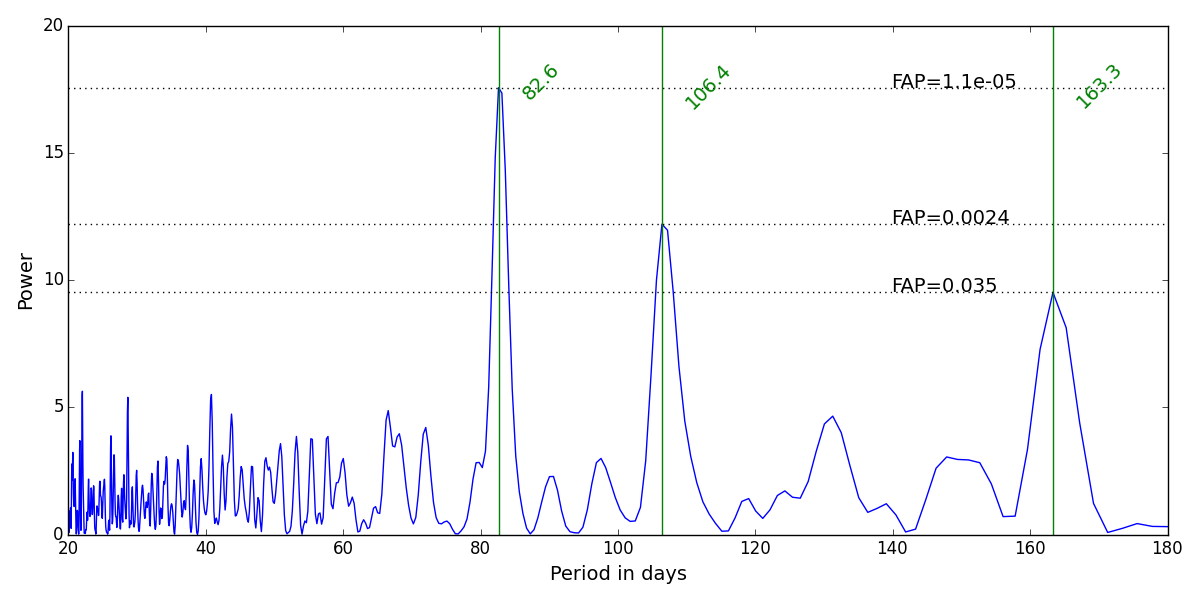
\includegraphics[scale=0.50]{Figures/asasnobin.png} \\
\end{center}
\caption{\examrevision{This is a periodogram calculated from the {\asas} database for {\prox} using 970 points of ``class A'' V-band
  data from the second aperture. In this periodogram no binning has been applied. The topmost 3 peaks at 82.6 days,
  106.4 days and 163.3 are shown and the corresponding FAP values marked in. Periods between 20 and 180 days are considered.}}
\protect\label{fig:asaspgram1}
\end{figure}

\begin{figure}[!htbp]
\begin{center}
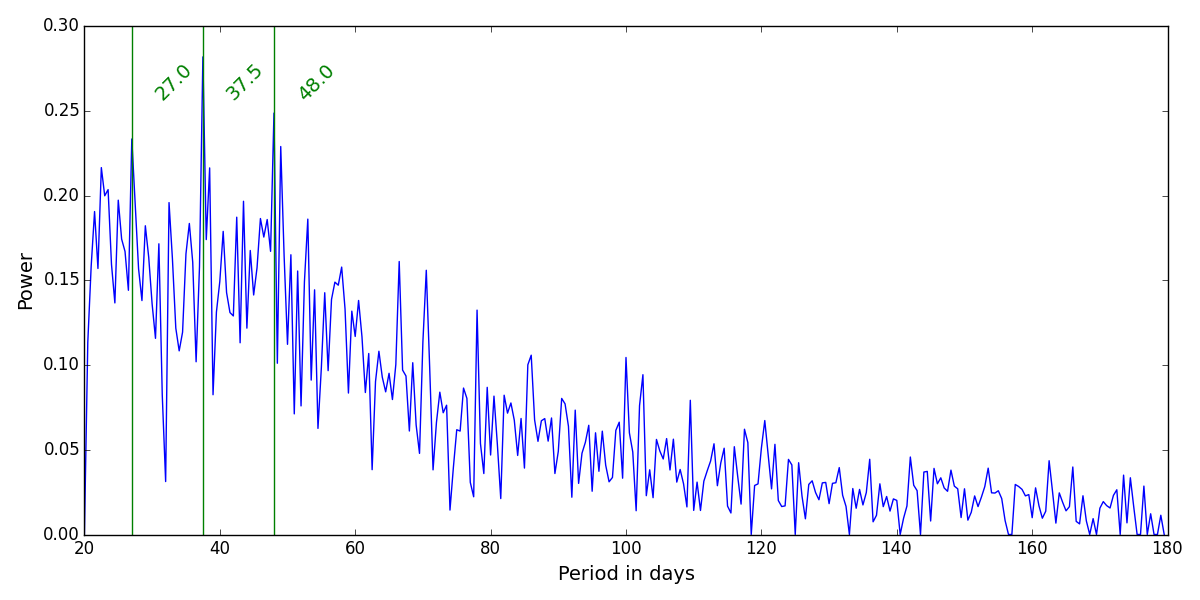
\includegraphics[scale=0.50]{Figures/asasnobinwf.png} \\
\end{center}
\caption{\examrevision{This figure displays the window function of the observation times of the periodogram displayed in
    Fig. \ref{fig:asaspgram1}. Note that that Y axis is on a considerably enlarged scale \examrevisiona{($\times 111$)} to that in
    Fig. \ref{fig:asaspgram1}.}}
\protect\label{fig:asaswf1}
\end{figure}

\examrevision{The 163.3-day period is close to double the 82.6-day period reported in the papers previously discussed
  and given here as the strongest peak and has a poorer FAP. It was therefore considered that the 82.6-day period was
  not likely to be a sub-harmonic of this. The window function of the observation times was also computed, \examrevisiona{using
  \textit{Period04}} and is displayed in Fig. \ref{fig:asaswf1}. Construction of a phase-folded light curve from the
  18-minute binned data yields Fig. \ref{fig:asaspflc}.}

As some of the observations were duplicated or apparently overlapping, these were initially binned to 1 day, in line
with several of the {\harps} results described in Section \ref{section:harpsper}. This reduced the number of points to
624. From the result the periodogram shown in Fig. \ref{fig:asaspgram2} was obtained. This appeared to clarify the peaks
by reducing the number with very short periods and enhancing the two major ones. Some binning appeared to be necessary
as some of the points had duplicated times. It appeared worthwhile to experiment with sizes of binning to see at what
point the result was optimal, in terms of yielding the strongest peaks with the lowest FAP and least extraneous peaks
and after trying various binning values between several days down to 1 minute, the optimal binning was found to be 18
minutes, yielding the periodogram shown in Fig. \ref{fig:asaspgram3}. Note that the scale of this is the same but the
figure has been made taller to accommodate the more powerful 82.6 day peak. The reduction of the points in the binning
to 18 minutes was found to be a much more modest reduction, to 924 observations from 970. The explanation of this
18-minute binning result may be related to the 3-minute exposure time for {\asas} 3 \citep{pojmanski01}.

\begin{figure}[!htbp]
\begin{center}
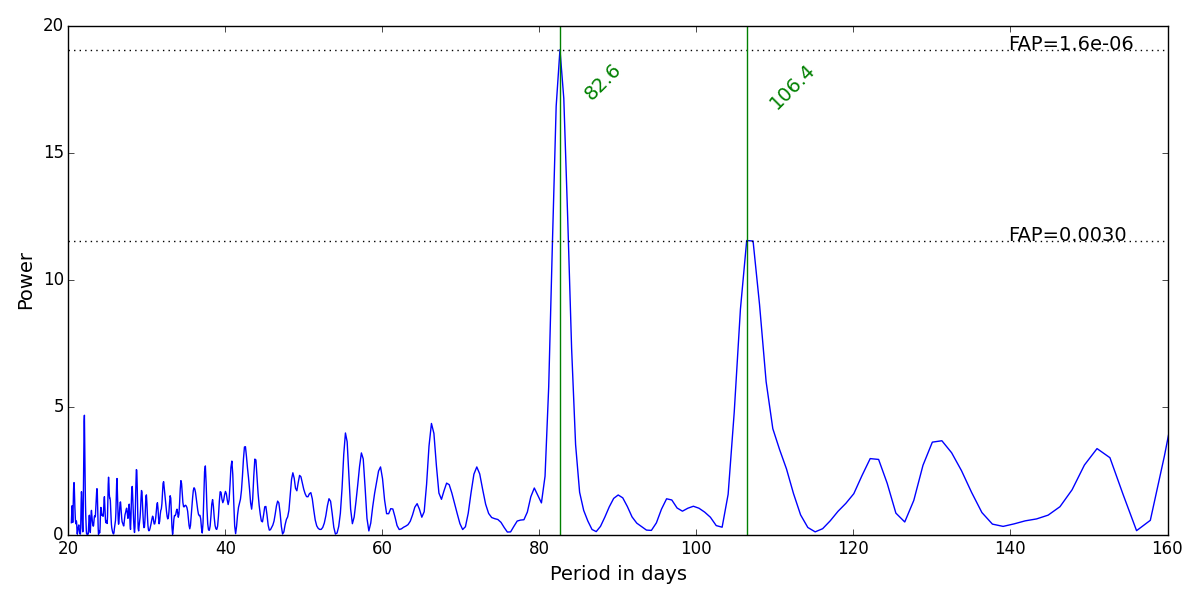
\includegraphics[scale=0.50]{Figures/asasbin1.png} \\
\end{center}
\caption{\examrevision{This is a periodogram calculated from the 624 points remaining (out of the original 970) after the ``Class A'' V-band data from the {\asas}
  database for {\prox}, using the second aperture, is binned to 1 day. Display is between 20 and 160 days.}}
\protect\label{fig:asaspgram2}
\end{figure}

\begin{figure}[!htbp]
\begin{center}
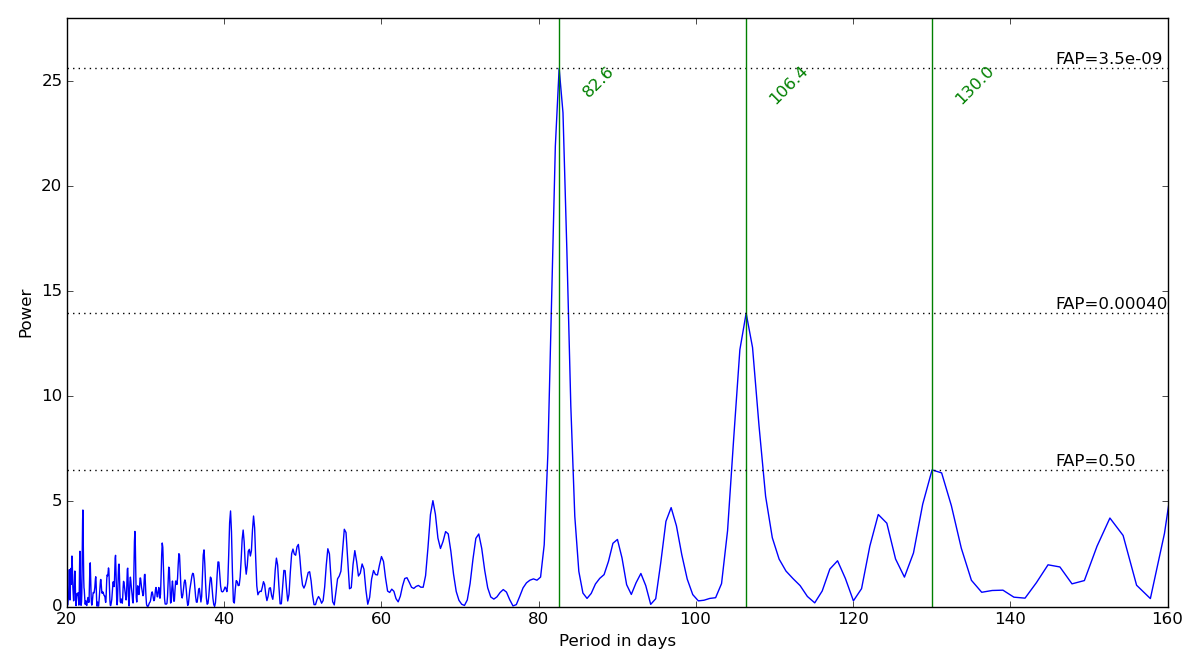
\includegraphics[scale=0.50]{Figures/asasbin18min.png} \\
\end{center}
\caption{\examrevision{This is a periodogram calculated from the 924 points remaining (out of the original 970) after the ``Class A'' V-band data from the {\asas}
  database for {\prox}, using the second aperture, is binned to 18 minutes. Display is between 20 and 160 days. Note
  that the Y axis of this is on the same scale as Fig. \ref{fig:asaspgram1} and Fig. \ref{fig:asaspgram2}.}}
\protect\label{fig:asaspgram3}
\end{figure}

\begin{figure}[!htbp]
\begin{center}
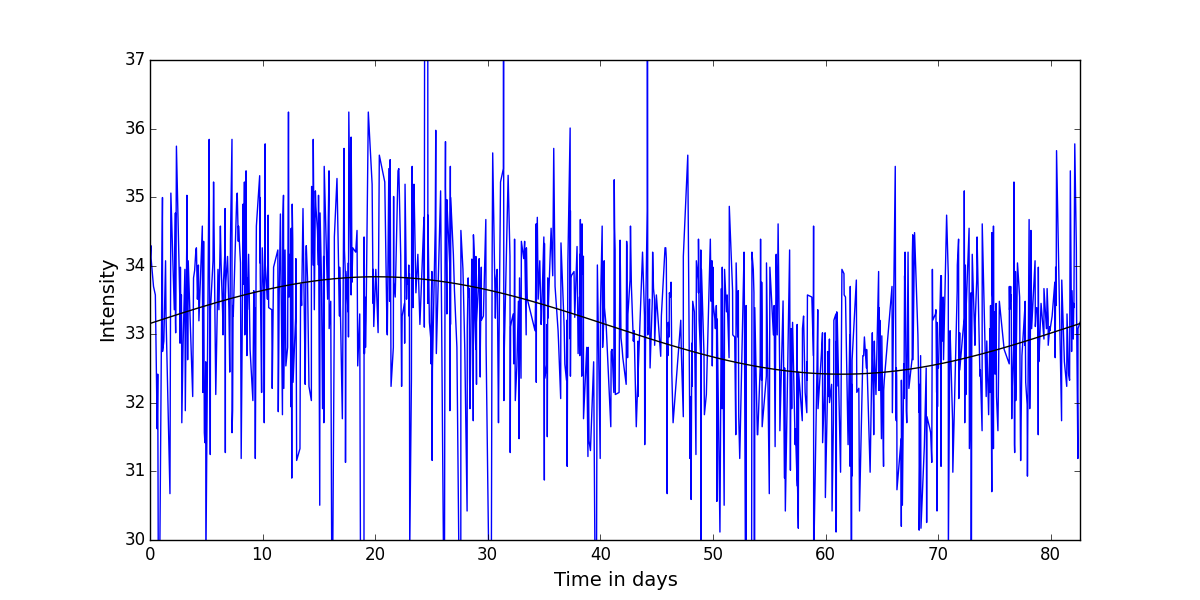
\includegraphics[scale=0.50]{Figures/asasb18minpf.png} \\
\end{center}
\caption{\examrevision{This illustrates the phase-folded light curve derived from the 924 points remaining (out of the
    original 970) after the ``Class A'' V-band data is binned to 18 minutes and folded to 82.6 days. Some extreme values
  are omitted in order to show the bulk of the data. A best-fit sinusoidal curve, shown in black, is fitted with baseline $ 33.12 \pm
  0.06 $, phase $ 0.49 \pm 0.02 $ and amplitude $ 0.71 \pm 0.09$. (A scatter plot was considered but the line plot
  appeared to be easier to follow in this instance, as opposed to Fig. \ref{fig:hstpf}.)}}
\protect\label{fig:asaspflc}
\end{figure}

Although the recommended aperture by {\asas} for {\prox} is the second aperture, it appeared valuable to compare the
three highest peaks from each of the apertures finding that nearly all the data gave a first peak of 82.6 days, a second
peak of 106.4 days and a much less significant third peak (over 0.5 FAP) of about 131 days in most cases. The results
are listed with no-binning, 1-day and 18-minute binnings in Table \ref{table:asasperiods}. Also considered were the
other grades of {\asas} data\footnote{These are mostly from ID 142944-6241.0.}, with a little under half of the Class A
data, 416 points and much higher error rating. All the periodograms from this lower quality data still showed a strong
peak of around 83 days. The results (for 18-minute binning only) are shown in Table \ref{table:lqasas}.

\begin{table}[!htbp]
\centering
\scalebox{0.8}{
\begin{tabular}{|l|l|r|r|r|}
\hline
Aperture & binning & Peak 1 & Peak 2 & Peak 3 \\
&&(days)&(days)&(days)\\\hline
1 & none & 83.1 & 106.4 & 131.3 \\
2 & none & 82.6 & 106.4 & 22.0 \\
3 & none & 82.6 & 106.4 & 131.3 \\
4 & none & 82.6 & 106.4 & 131.3 \\
5 & none & 82.6 & 106.4 & 131.3 \\\hline
1 & 1 day & 82.6 & 106.4 & 110.6 \\
2 & 1 day & 82.6 & 106.4 & 22.0 \\
3 & 1 day & 82.6 & 106.4 & 130.0 \\
4 & 1 day & 82.6 & 106.4 & 42.6 \\
5 & 1 day & 82.6 & 106.4 & 42.4 \\\hline
1 & 18 min & 83.1 & 106.4 & 131.3 \\
2 & 18 min & 82.6 & 106.4 & 130.0 \\
3 & 18 min & 82.6 & 106.4 & 130.0 \\
4 & 18 min & 82.6 & 106.4 & 130.0 \\
5 & 18 min & 82.6 & 106.4 & 131.3 \\\hline
\end{tabular}}
\caption{Summary of three strongest periods taken from Class A values in {\asas} dataset for {\prox} from all apertures based upon magnitudes measured
  between December 2000 and September 2009. Results are shown for the raw data. 1-day binning and 18-minute binning.}
\protect\label{table:asasperiods}
\end{table}

\begin{table}[!htbp]
\centering
\scalebox{0.75}{
\begin{tabular}{|l|r|l|r|l|r|l|}
\hline
Aperture & Peak 1 & FAP & Peak 2 & FAP & Peak 3 & FAP \\
& (days) && (days) && (days) &\\\hline
1 & 83.1 & 0.0067 & 105.8 & 0.33 & 127.4 & 0.82 \\
2 & 83.1 & 0.03 & 105.8 & 0.43 & 127.4 & 0.61 \\
3 & 83.1 & 0.038 & 105.8 & 0.31 & 128.7 & 0.89 \\
4 & 84.1 & 0.1 & 105.8 & 0.21 & 128.7 & 0.93 \\
5 & 84.1 & 0.0024 & 105.8 & 0.0028 & 82.5 & 0.0033 \\\hline
\end{tabular}}
\caption{Summary of three strongest periods taken from Class B and lower quality values in {\asas} datasets for {\prox}
  based upon magnitudes measured between December 2000 and September 2009 binned to 18 minutes.}
\protect\label{table:lqasas}
\end{table}

It was noticeable that all of the Lomb-Scargle routines listed in Appendix \ref{chapter:lsroutines} gave exactly
the same results (apart from differences to scaling of the power) with all the {\asas} data, including the lower quality
data. This was in contrast to the spectroscopic results discussed in later chapters of this \paperorthesis.

A search was made for very long periods up to the period spanned by the data in each case, however no strong periods
could be found, in particular nothing close to the 442 days reported in \citet{cincunegui07}\footnote{No such period was
  found in the {\hst} or spectroscopic results either.}.

\section{HST}
\protect\label{section:hst}

\examrevision{As another source of photometric results, periodograms} were derived from the {\hst} data discussed in
\examrevision{\citet{benedict92} and in \citet{benedict98}} consisting of 171 points obtained between July 1995 and
January 1998, later enhanced so the last 18 points extended to January 2001. \examrevision{The data used a filter
  centred on 583nm with 234nm FWHM \citep{benedict98}}. Three times were actually duplicated and eliminating the
duplications \examrevision{(taking the mean value)}, it was possible to obtain the periodogram in
Fig. \ref{fig:hstb4min}.

\begin{figure}[!htbp]
\begin{center}
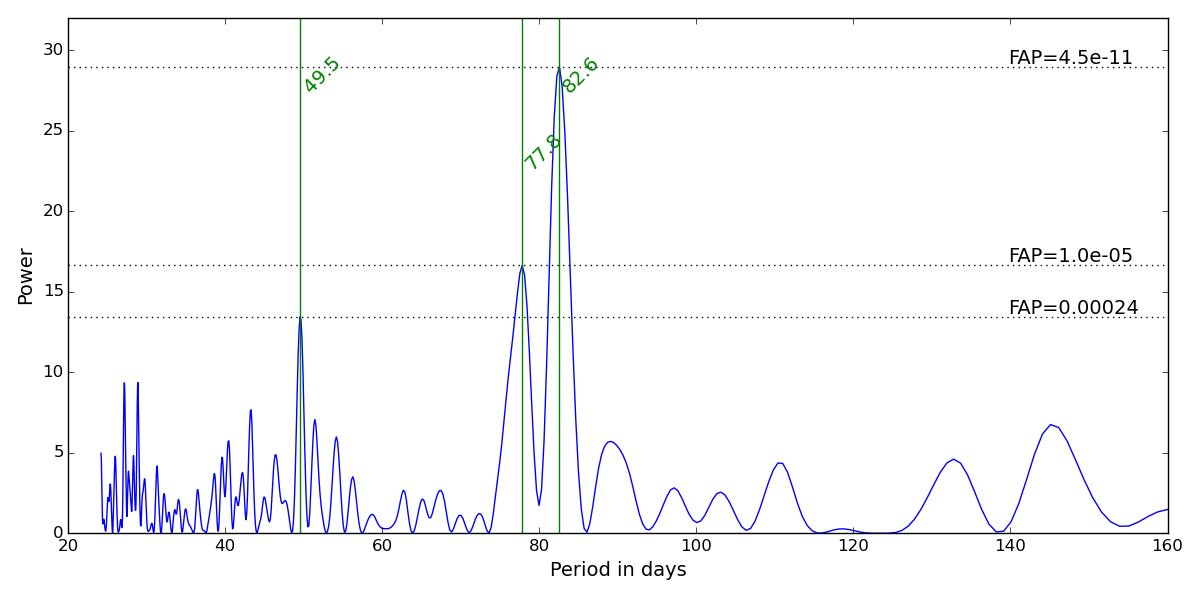
\includegraphics[scale=0.50]{Figures/hstb4min.png} \\
\end{center}
\caption{This is a periodogram \examrevision{derived} from the {\hst} data discussed in \citet{benedict98} between July 1995 and
  January 1998 plus some additional points up to January 2001 examining periods showing the three highest peaks and with
  the FAPs marked in. \examrevision{This has been binned to 4 minutes to eliminate 3 duplicated times.}}
\protect\label{fig:hstb4min}
\end{figure}

\begin{figure}[!htbp]
\begin{center}
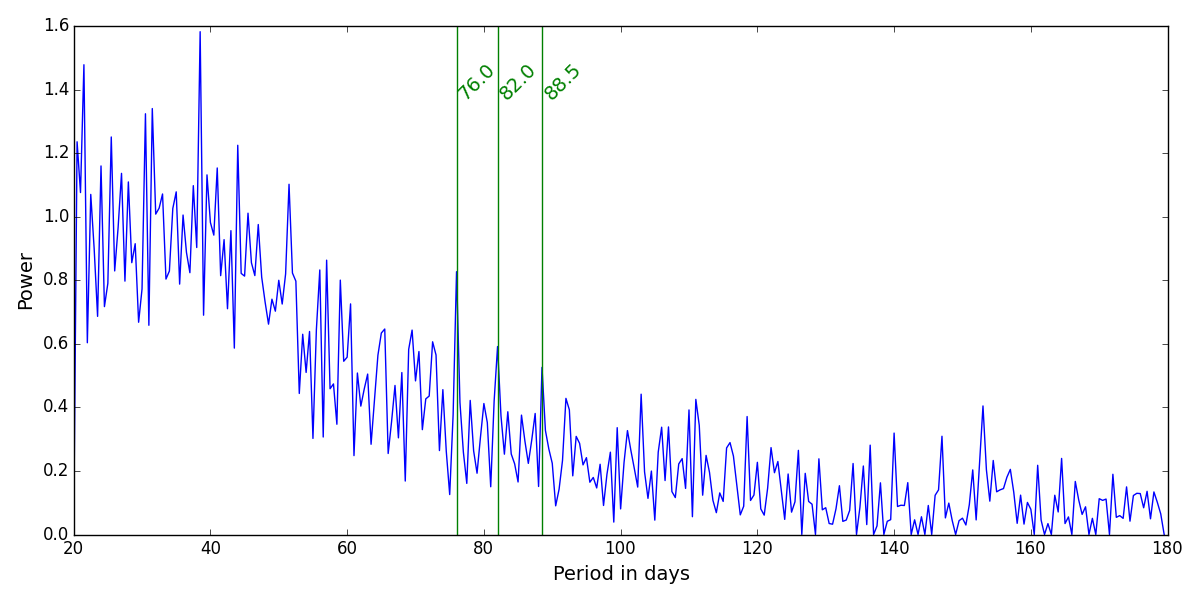
\includegraphics[scale=0.50]{Figures/hstwinfunc.png} \\
\end{center}
\caption{\examrevision{Window function for the {\hst} observation times highlighting three peaks close to the 77.8 day
    and 82.6 day peaks observed in Fig. \ref{fig:hstb4min}. Note the Y scale in this figure is considerably enlarged by
    comparison with that figure.}}
\protect\label{fig:hstwf}
\end{figure}

Again, as with the {\asas} data, all the Lomb-Scargle routines listed in Appendix \ref{chapter:lsroutines}
\examrevision{gave almost identical periodograms} (other than the scaling of the power). \examrevision{A phase-folded
  light curve of this is displayed in Fig. \ref{fig:hstpf}. Examination of the window function of these observation
  times, \examrevisiona{using \textit{Period04},} gave the result shown in Fig. \ref{fig:hstwf}.}. \examrevisiona{It
  would appear from the window function that the peak of around 78 days in Fig. \ref{fig:hstb4min} could well be due to
  this peak in the window function.}

\begin{figure}[!htbp]
\begin{center}
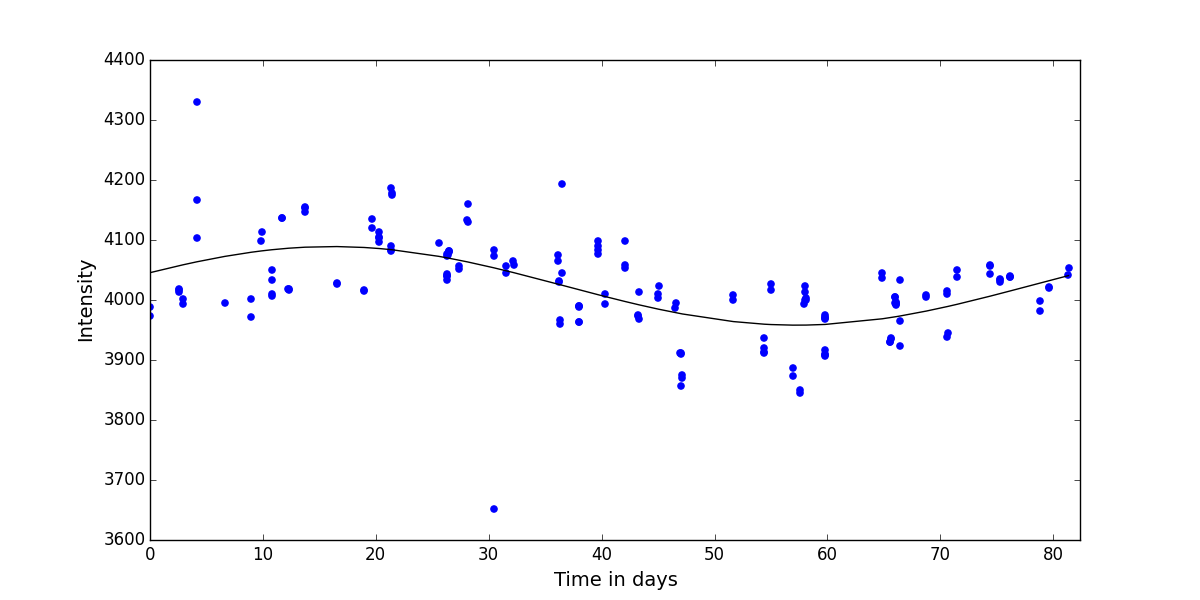
\includegraphics[scale=0.50]{Figures/hstpfold.png} \\
\end{center}
\caption{\examrevision{Phase-folded light curve, folded to 82.6 days, of {\hst} data discussed in \citet{benedict98},
    with best-fit sine curve fitted, shown in black. This has amplitude $ 65 \pm 7 $, a phase of $ 0.45 \pm 0.02 $ and a base level of
    $4024 \pm 5$. (A line plot was considered but the scatter plot appeared to be easier to follow in this instance, as opposed to Fig. \ref{fig:asaspflc}).}}
\protect\label{fig:hstpf}
\end{figure}

\section{Summary of photometric results}
\protect\label{section:summphotometric}

The period at 82.6 days is clearly as a strong, very low-FAP peak in both the {\asas} and {\hst} data. It is almost
certainly the rotation period of {\prox}, seemingly with a small error bar, although some investigations in Section
\ref{section:asasfap} were undertaken partly to investigate this.

It also provides a convenient benchmark for assessing the accuracy and reliability of the other, less clear
spectroscopic methods investigated in Chapter \ref{chapter:proxima} based on the {\ha} line.

The {\asas} data, including the lesser quality data also included a strong peak at 106.4 days but this was not seen on
the {\hst} data. The former, however, has observation times much more constrained by the time of year and it is
noticeable that:

\begin{center}

$ \frac{1}{\frac{1}{82.6} - \frac{1}{365.25}} = 106.7 $

\end{center}

There remains the strong 77.8-day period seen in the {\hst} data but not in the {\asas} data to be accounted for,
\examrevisiona{but this would appear to correspond to a close-by peak in the window function illustrated in Fig. \ref{fig:hstwf}, so}
\examrevision{this is quite possibly an alias thrown up by the observation times.}
